\section{Demo}

\subsection{To-do List}
Al fine di dare una dimostrazione pratica dell'utilizzo del framework presentato nel paragrafo antecedente, verranno sviluppati due esempi significativi di bubble interattiva.\\
Il primo è una bubble contenente una lista di cose da fare chiamata To-do list.\\
La struttura di questa bubble interattiva sarà analoga a quella presentata nel framework relativamente alla bubble generica e sarà quindi composta da tre parti:
\begin{itemize}
	\item una parte di view tramite la quale l'utente potrà interagire con il sistema, segnando come completate, aggiungendo o rimuovendo voci nella lista;
	\item una parte avente funzione di controller incaricata di ricevere i segnali dall'interfaccia grafica, riconoscerli ed inviarli alla parte di modello in cui verranno gestiti, e viceversa di ricevere i segnali dalla parte di modello e renderizzarli tramite la GUI;
	\item una parte di modello con il compito di gestire la business logic dell'applicativo bubble To-do list.
\end{itemize}
Conformemente a quanto riportato nell'\AnalisiDeiRequisiti{} saranno possibili le seguenti interazioni con il sistema:
\begin{itemize}
	\item creazione di una nuova lista tramite la creazione di una bubble;
	\item aggiunta di elementi alla lista;
	\item rimozione di elementi dalla lista;
	\item possibilità di aggiungere un reminder come notifica.
\end{itemize}

\subsubsection{Package To-do List}

Il package della To-do List segue il pattern Model-View-Controller (MVC), e dunque contiene i package View, Controller e Model. Il package View contiene tutti gli elementi grafici della To-do List e forma la GUI visibile agli utenti della bubble. Il package Model permette operazioni sui dati riguardanti la To-do List e le notifiche ad essi associate salvati sia nella Bubble Memory sia nel DataBase attraverso il package DB Gateway. Il package Controller è dedicato alla ricezione degli input dagli attori permettendo agli stessi l'interazione con i dati contenuti nel Model e l'aggiornamento della View.

%\begin{figure}[H]
%	\centering
%	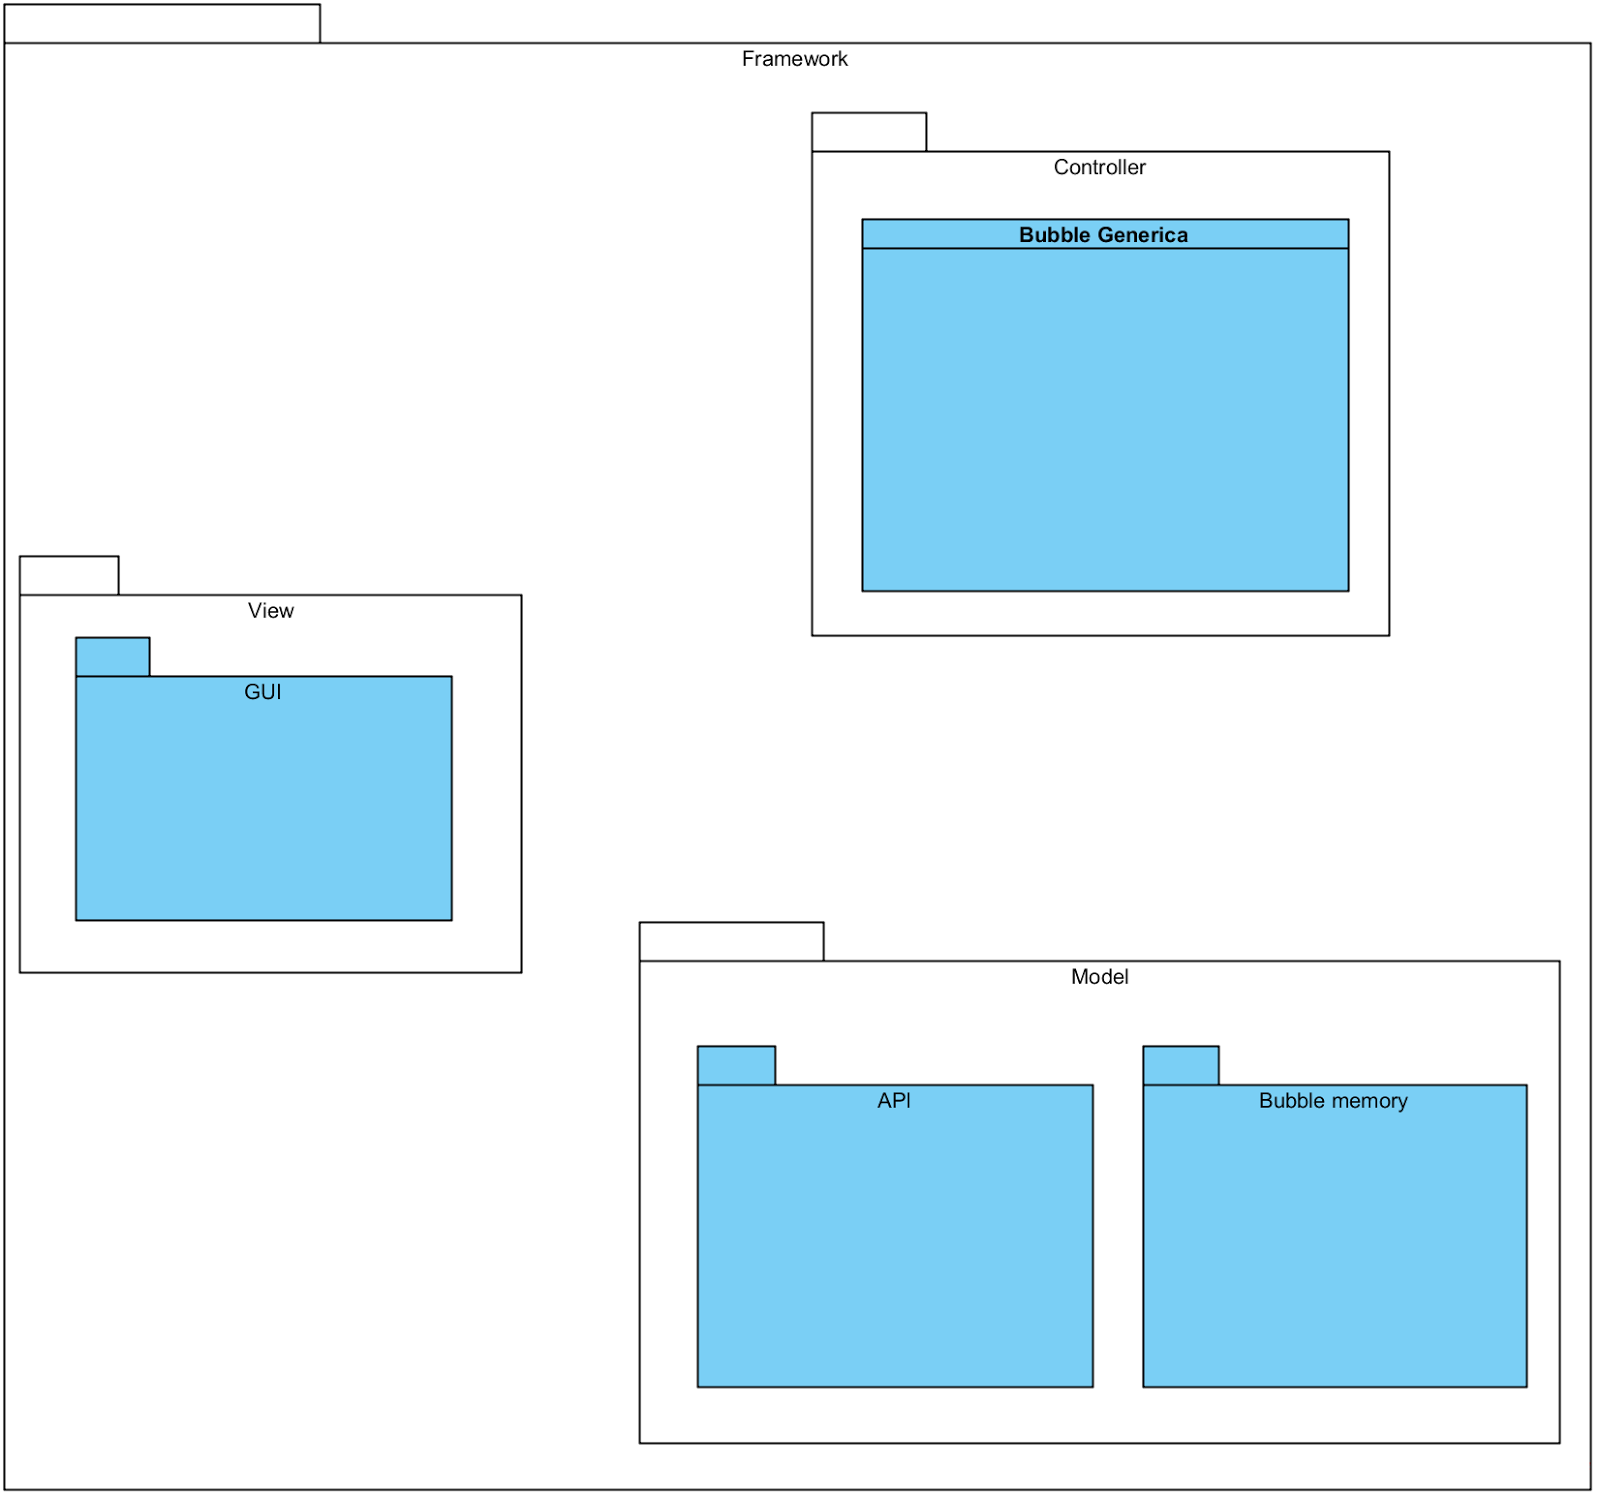
\includegraphics[width=15cm]{../../documenti/SpecificaTecnica/diagrammi_img/framework.png}
%	\caption{Package To-do List}
%\end{figure}

\begin{samepage}
\paragraph{View}\mbox{}\\
%\begin{figure}[H]
%	\centering
%	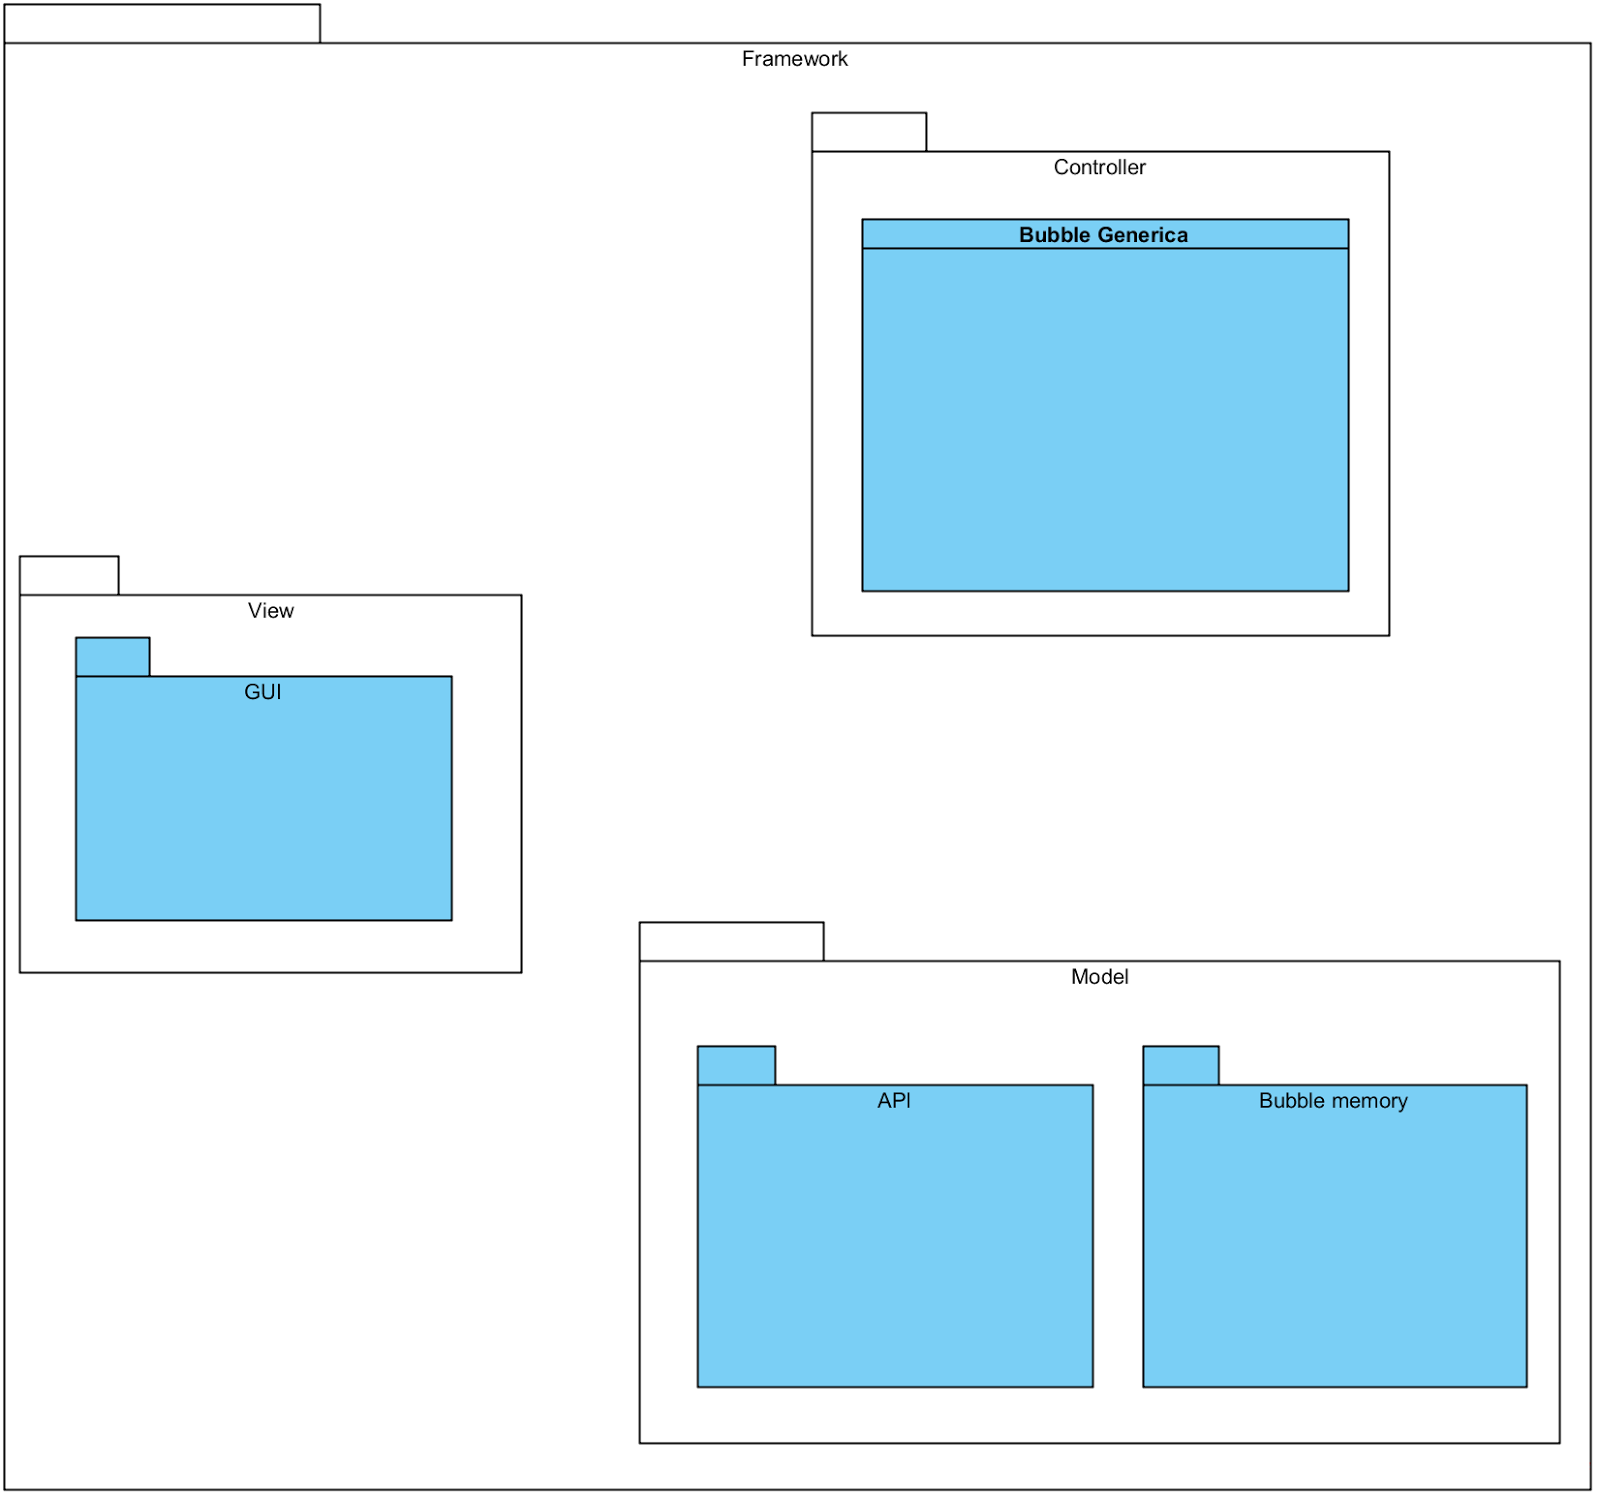
\includegraphics[width=15cm]{../../documenti/SpecificaTecnica/diagrammi_img/framework.png}
%	\caption{View}
%\end{figure}
\end{samepage}

\paragraph{Model}\mbox{}\\
Il package Model gestisce i dati contenuti nella bubble memory e nel database associato tramite i package Bubble Memory e DB Gateway. Permette inoltre di impostare notifiche tramite il package Notifica. I dati sono rappresentati dal package List Items ovvero le liste contenute nella bubble To-do List. List Items Container definisce le liste, formate da oggetti della classe List Item, cioè singole voci delle liste. 
%\begin{figure}[H]
%	\centering
%	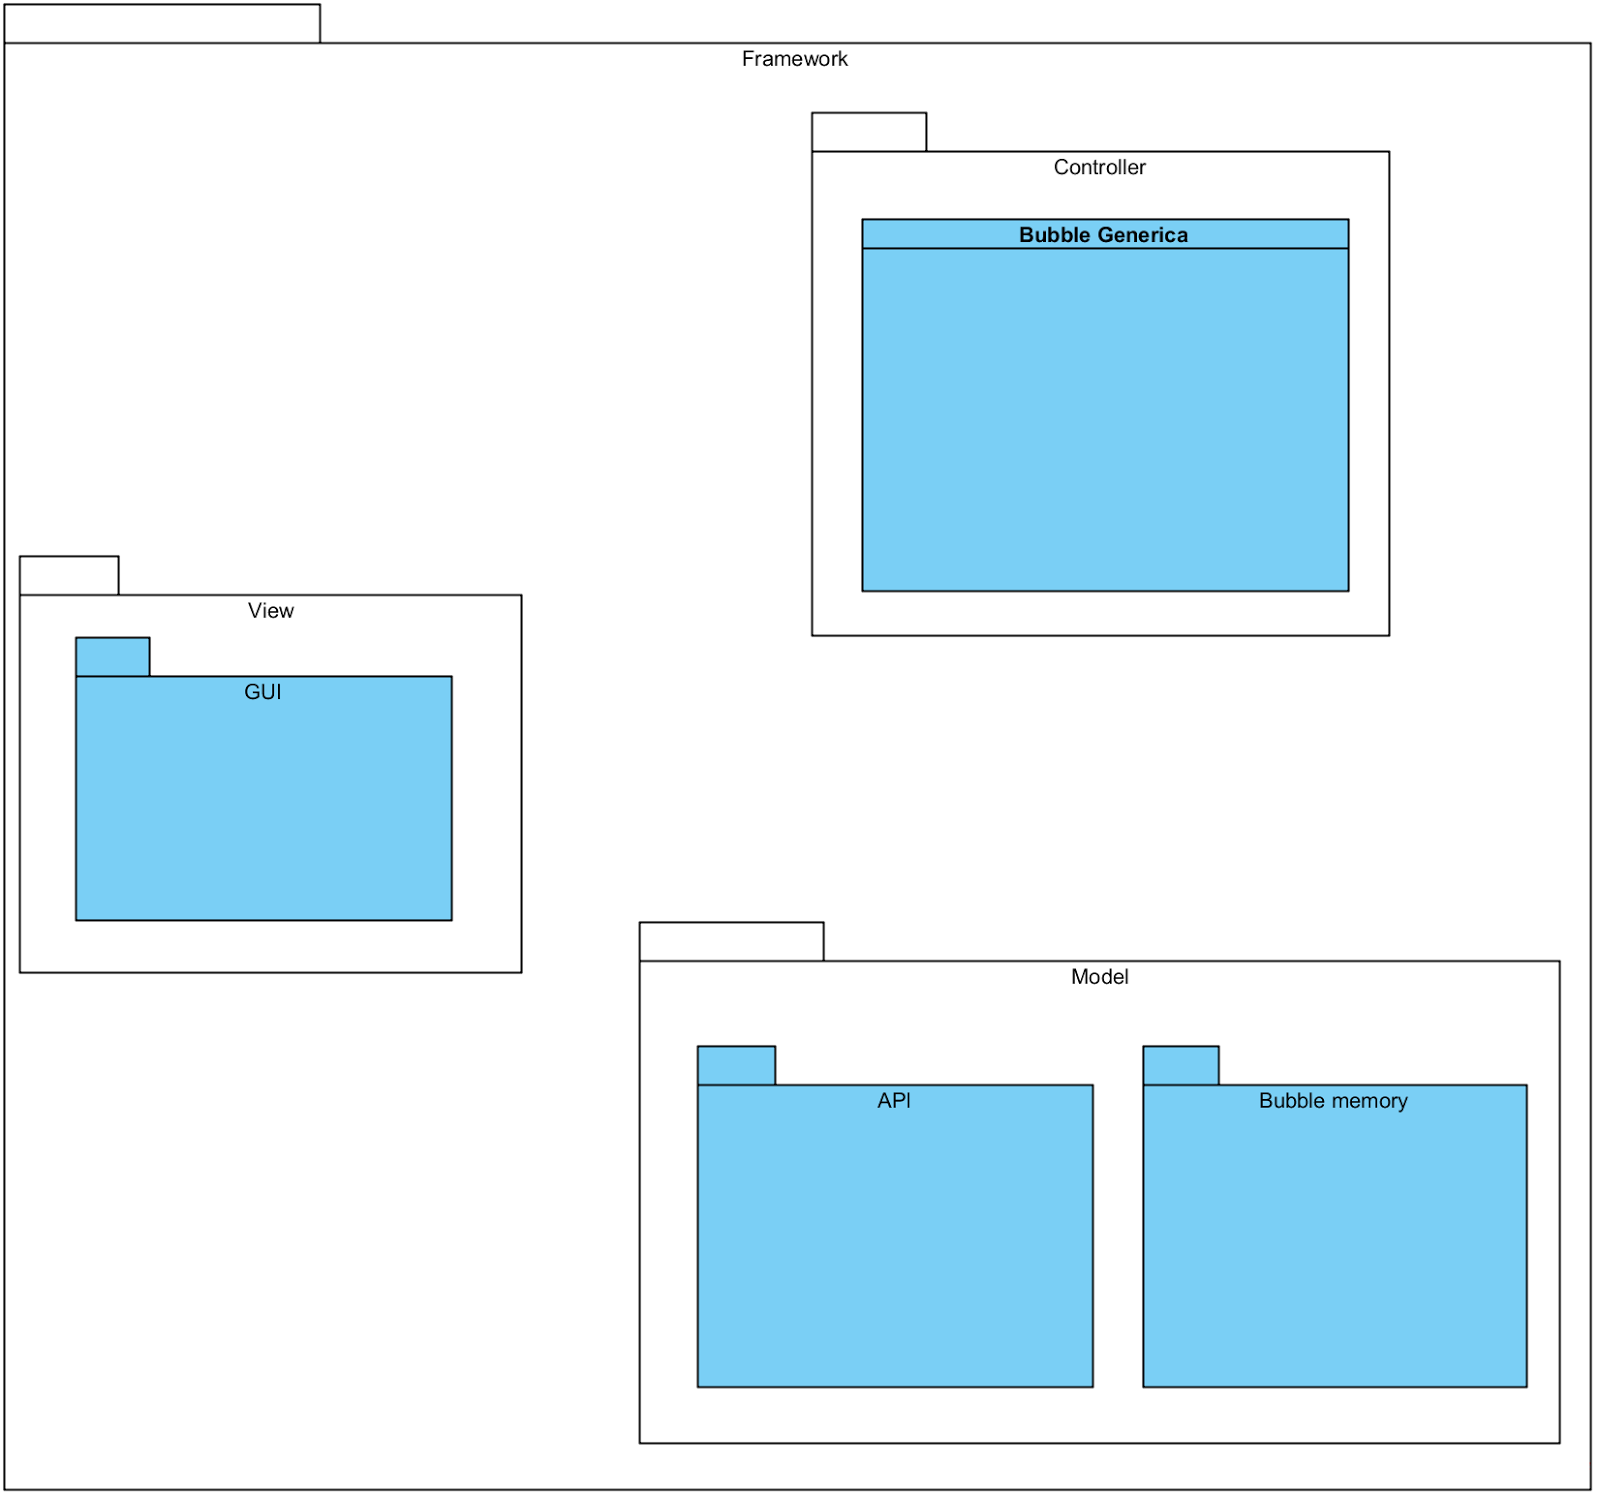
\includegraphics[width=15cm]{../../documenti/SpecificaTecnica/diagrammi_img/framework.png}
%	\caption{Model}
%\end{figure}

%\begin{figure}[H]
%	\centering
%	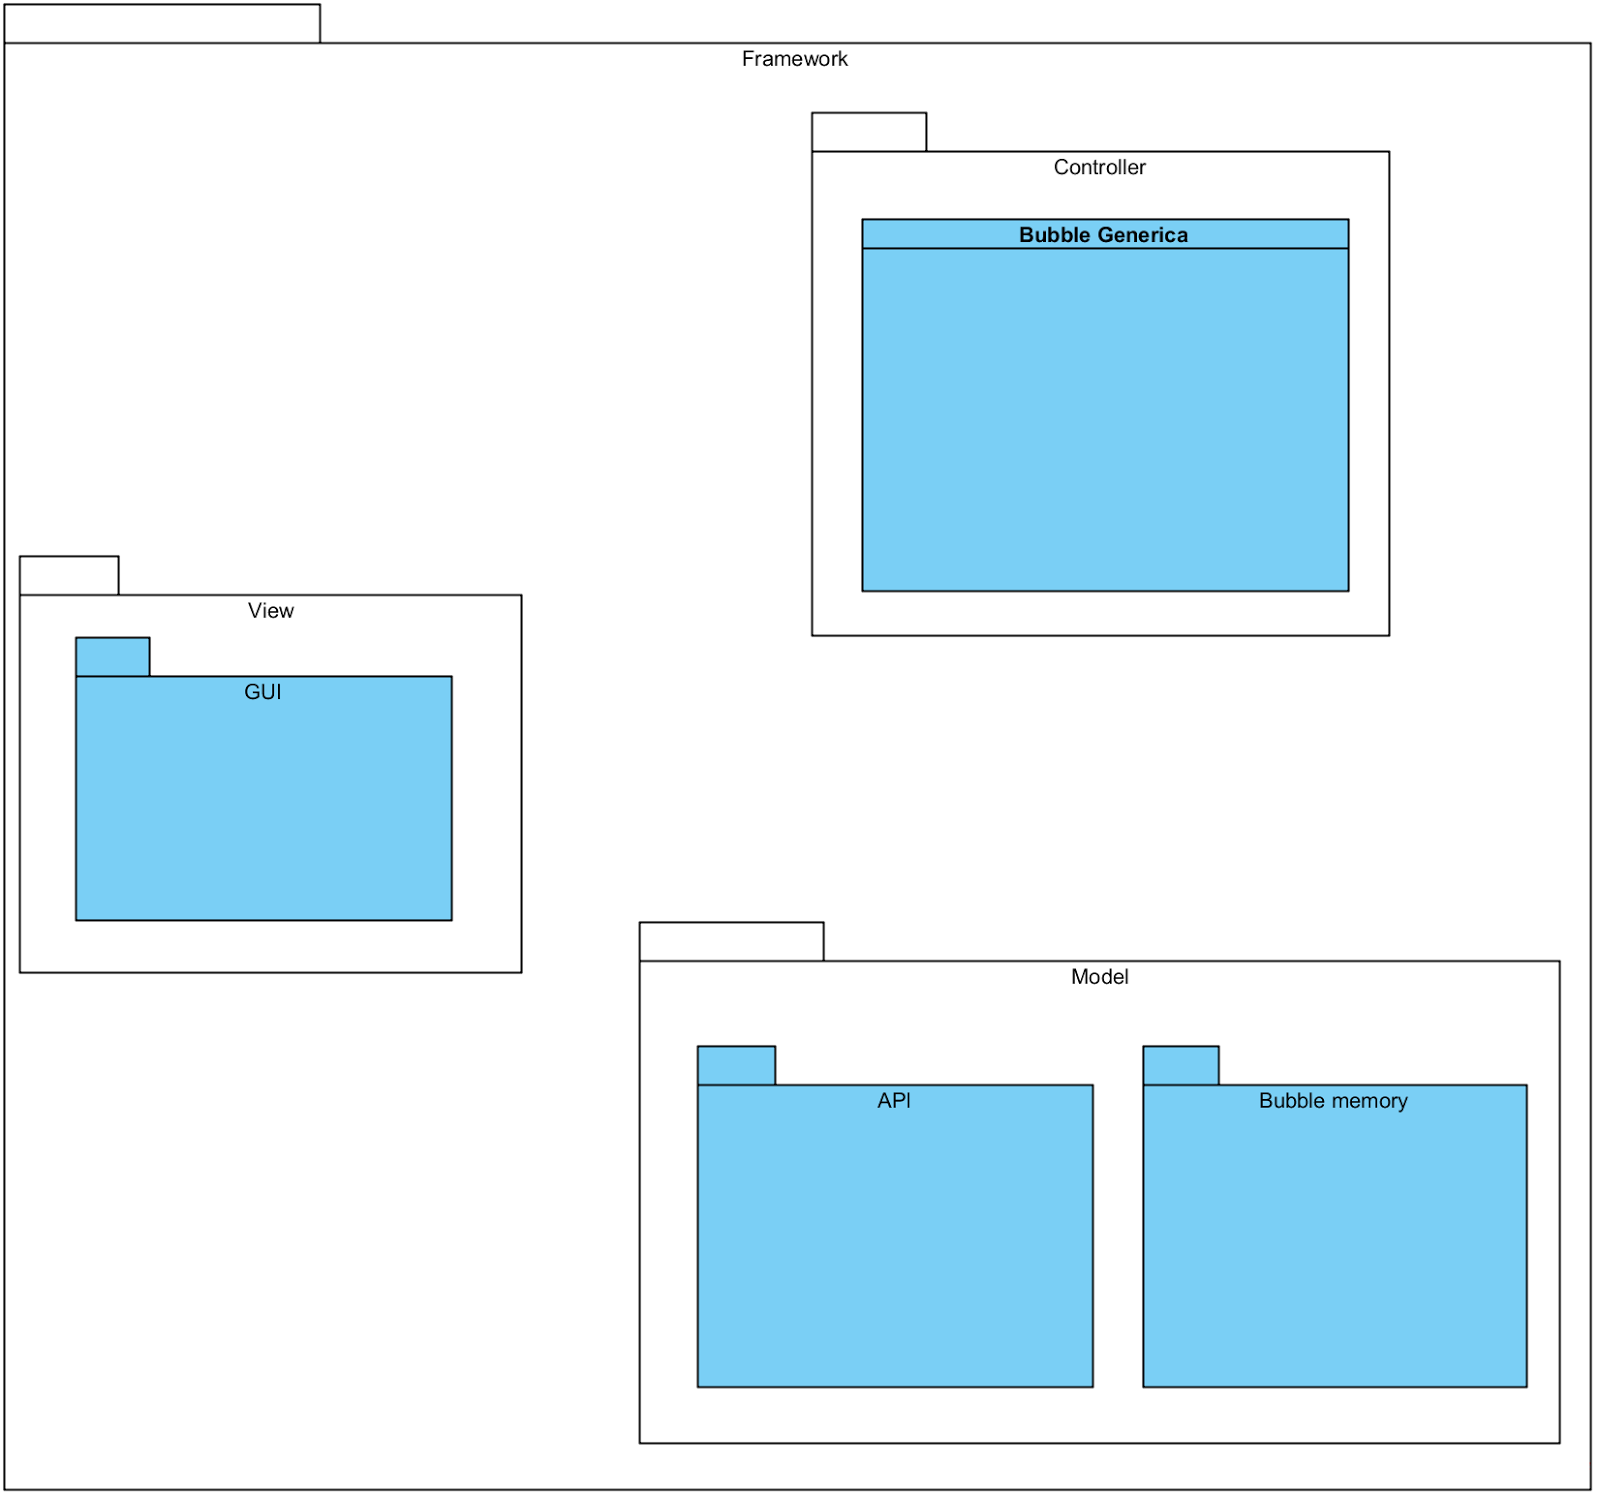
\includegraphics[width=15cm]{../../documenti/SpecificaTecnica/diagrammi_img/framework.png}
%	\caption{List Items}
%\end{figure}

\subparagraph{Model::List Items::List Item}\label{todo-item}\mbox{}\\
\textbf{Descrizione:}\\
La classe List Item rappresenta un'entrata per la To-do list.\\
\textbf{Utilizzo:}\\
L'utilizzo di questa classe è quello di fornire un'implementazione per le entrate della bubble To-do list in modo da poter creare o eliminare voci dalla lista, essere segnate come completate o settare un reminder.\\

\subparagraph{Model::List Items::List Item Container}\mbox{}\\
\textbf{Descrizione:}\\
La classe List Item permette la gestione di una collezione di voci della To-do list definite dalla classe List Item.\\
\textbf{Utilizzo:}\\
Questa classe offre la possibilità di aggiungere, rimuovere e restituire elementi da una collezione di elementi della To-do list.\\

\subparagraph{Model::DB Gateway::DB Gateway}\mbox{}\\
\textbf{Descrizione:}\\
La classe DBGateway permette agli attori di interagire con la To-do list. La classe si occupa inoltre di inviare le notifiche impostate sui ListItem. \\
\textbf{Utilizzo:}\\
Questa classe permette agli attori la manipolazione dei ListItem, per segnare come completate le voci della lista, settare notifiche, creare ed eliminare ListItems dalla To-do list.\\